
%(BEGIN_QUESTION)
% Copyright 2014, Tony R. Kuphaldt, released under the Creative Commons Attribution License (v 1.0)
% This means you may do almost anything with this work of mine, so long as you give me proper credit

Calculate all voltages and all currents in this circuit, given the component values and the number of turns in each of the transformer's windings:

$$\includegraphics[width=15.5cm]{i01239x01.eps}$$

\underbar{file i01239}
%(END_QUESTION)





%(BEGIN_ANSWER)

$V_R =$ 750 V

$I_R =$ 340.9 mA

\vskip 5pt

$V_{source} =$ 50 V

$I_{source} =$ 5.114 A

%(END_ANSWER)





%(BEGIN_NOTES)

This question checks students' ability to relate the winding ratio to voltage and current ratios in a transformer circuit.  The symbolism here is common in Europe, but not so common in the United States.

%INDEX% Electronics review: transformer ratios

%(END_NOTES)


